% das Papierformat zuerst
\documentclass[a4paper, 11pt]{article}

% deutsche Silbentrennung
\usepackage[ngerman]{babel}

% wegen deutschen Umlauten
\usepackage[ansinew]{inputenc}

% Grafikpaket laden
\usepackage{hyperref}
\usepackage{graphicx}

% wir wollen auf jeder Seite eine Ueberschrift
\pagestyle{headings}

% hier beginnt das Dokument
\begin{document}

% Inhaltsverzeichnis anzeigen
\tableofcontents

\setlength{\parindent}{0pt}

% Kapitel soll auf naechster Seite beginnen
\newpage

\section{Einleitung}

Ich habe angefangen mit der Programmiersprache Julia zu arbeiten, um zu testen, ob diese leicht zu lernen, einfach zu parallelisieren und dabei noch schnell ist, fuer verschiedene numerische Anwendungen. 
In meinen anfaenglichen Beispielen, vergleiche ich Julia mit Python. 
Python ist eine universelle, blicherweise interpretierte h\"ohere Programmiersprache. Sie will einen gut lesbaren, knappen Programmierstil f\"ordern.So wird beispielsweise der Code nicht durch geschweifte Klammern, 
sondern durch Einrckungen strukturiert.(Wikipedia)
Julia hingegen ist eine h\"ohere High-Performance-Programmiersprache, welche vor allem f\"ur numerisches und wissenschaftliches Rechnen entwickelt wurde, w\"ahrend sie dennoch als eine General Purpose Language verwendet werden kann, 
bei gleichzeitiger Wahrung einer hohen Ausfhrungsgeschwindigkeit.(Wikipedia)
Julia ist eine Programmiersprache, die auf der einen Seite sehr einfach zu lernen ist und trotzdem eine hohe Ausfhrungsgeschwindigkeit hat. Man kann sehr gut numerisch mit Julia arbeiten. Alle n\"otigen Methoden sind vorimplementiert und 
die zugeh\"orige Doku ist bis jetzt sehr bersichtlich aber trotzdem gut verst\"andlich. Zudem soll mit Julia die Parallelisierung von Programmen einfacher sein als in Python. Dies ist fr diese Tests nicht wichtig, aber kann im weiteren Verlauf
noch wichtig werden.
Die mathematischen Laufzeitvortest die ich durchgefhrt habe, basieren auf den Angaben der Webseite von \url{http://julialang.org/} und selbst ausgetesteten numerischen Funktionen wie beispielsweise der LU Zerlegung. Ich konnte dabei best\"atigen, 
dass Julia gr\"o\ss{}tenteils schneller ist als Python.
Die Ausnahme, die ich best\"atigen konnte, war ein \url{https://github.com/kbarbary/website/blob/master/posts/julia-vs-numpy-arrays.rst} von Kale Barbary berprft in dem es um einen Fall geht, in dem Python teilweise schneller ist als Julia. 
Dieses Ergebnis konnte ich best\"atigen.

\section{Gegebenheiten}
Ich arbeite mit Python 3.5 in der Umwicklungsumgebung Pycharm. In Julia arbeite ich mithilfe Des Jupyter Notebooks in der Juliaversion 0.4.7.

\section{Was sind Iterative L\"oser?}
Iterative L\"oser werden benutzt um gro\ss{}e lineare Gleichungen in der Form: \(Ax=b\) aufzul\"osen. Sie berechnen eine Ann\"aherung an die L\"osung. Dadurch sind sie viel schneller als direkte L\"osungsverfahren f\"ur lineare Gleichungen. 
Dies gilt vor allem, wenn \(A\) eine d\"unn besetzte Matrix ist. Das bedeutet das \(A\) viele Nulleintr\"age hat.
Die grundlegende Idee eines iterativen L\"osers ist durch eine immer genauere Ann\"aherung an die L\"osung bis zu einem bestimmtem Fehler eine m\"oglichst genaue L\"osung herauszufinden. 
Dieser Fehler ist der Unterschied zwischen den letzten beiden Iterationen. Dieser soll kleiner sein als ein Residuum $\epsilon$.
Um dies Umzusetzen gibt es verschiedene Verfahren. Ich habe im Grunde mit drei verschiedenen Verfahren gearbeitet: Dem Richardson Verfahren, dem Jacobi Verfahren und dem Gauss-Seidel Verfahren. 
Zudem habe ich das Jacobi Verfahren und das Gauss-Seidel Verfahren optimiert.

\newpage

\section{Verfahren}

\subsection{Wie ist der grundlegende Aufbau der Verfahren?}
Verfahrenabh\"angig wird die Iterationsmatrix M aus der Matrix A gebildet. Solange die Abbruchbedingung nicht erfllt ist,wird immer wieder die Gleichung: \begin{equation}x_{k+1}=Mx_{k}+b\end{equation}

\subsection{Richardson:}
Richardson ist das am einfachsten umzusetzende Verfahren. Es ist aber in der Praxis kaum anwendbar, da es im Vergleich zu den anderen Verfahren sehr viele Iterationen braucht und oft nicht konvergiert.
Die Idee ist, dass man mit der Fixpunktgleichung 
\begin{equation}
x=(I-A)x+b
\end{equation}  (I ist eine Einheitsmatrix mit gleichen Dimensionen wie A)arbeitet. Daraus ergibt sich das 
\begin{equation}
M_{Rich}=I-A
\end{equation}
ist. Um dieses Verfahren zu verbessern kann man mit Vorkonditionierern arbeiten. Das bedeutet, dass man grunds\"atzlich nicht die Gleichung \(Ax=b\) l\"ost, sondern die Gleichung 
\begin{equation}
BAX=Bb
\end{equation}
loesen. Durch intelligentes w\"ahlen von \(B\) kann man das Gleichungssystem so sehr vereinfachen. B sollte man so w\"ahlen, dass es nah an \(A^{-1}\) ist oder die Gleichung einfacher zu berechnen wird. Im speziellen Fall bei Richardson, dass \(B=I\) ist,
also die Matrix einfacher zu berechnen macht. Daraus folgt, dass ich \(M=I\) w\"ahlen kann. Deswegen ver\"andert sich auch die Iterationsberechnung:
\begin{equation}
x_{k+1}=Mx_{k}+Bb
\end{equation}

\subsection{Verfahren mit Matrix Splitting(Jacobi, Gauss-Seidel)}
Die Idee beim Matrix Splitting ist, dass man die Matrix aufteilt in einen Teil der einfach zu invertieren ist und einen der schwer zu invertieren ist. Hier teilt man die Matrix als erstes in eine untere Dreiecksmatrix \(L\), 
die Diagonalmatrix \(D\) und die obere Dreiecksmatrix \(U\). Daraus folgt, dass \(A = L+D+U\). Dies bestimmt nun den Vorkonditionierer \(B\).
F\"ur das Jacobi Verfahren w\"ahle ich \(B_{Jac}=D^{-1}\). Daraus folgt das
\begin{equation}
M_{Jac}=I-D^-1A.
\end{equation}
Da man mit desto mehr Informationen auch niedrigere Iterationszahlen erreichen kann benutzt man f\"ur das Gauss-Seidel Verfahren \(B_{GS} = (L+D)^-1\). Daraus folgt 
\begin{equation}
M_{GS} = I-(L+D)^{-1}A \Leftrightarrow M_{GS} = -(L+D)^{-1}U.
\end{equation} Vom Gauss-Seidel Verfahren gibt es auch andere Varianten wie den Backward Gauss Seidel bei dem 
\begin{equation}
  M_{BGS} = -(U+D)^{-1 }L
\end{equation} oder den Symmetrischen Gauss Seidel 
\begin{equation}
M_{SGS}= M_{GS}M_{BGS},
\end{equation} die ich aber nicht implementiert habe, da man keine gro\ss{}artige Verbesserung von diesen erwarten kann.(Das vielleicht noch mehr erkl\"aren!)

\subsection{Wann funktionieren die Verfahren?}
Um zu beurteilen ob eines dieser Verfahren funktioniert, muss ich \"uberpr\"ufen, ob dieses konvergiert. Ausschlaggebend daf\"ur ist der Spektralradius. Dieser wird durch die Eigenwerte der Iterationsmatrix M bestimmt.
Da ich mich daf\"ur entschieden habe mit der Maximumsnorm zu arbeiten ist der gr\"o\ss{}te Eigenwert ausschlaggebend. Wenn dieser Wert kleiner als eins ist konvergiert das Verfahren. 
Je kleiner der Spektralradius ist, desto schneller konvergiert das Verfahren. (Wahrscheinlich besser erst nach den Verfahren, dann ist das mit dem Spektralradius leichter).

\subsection{Aufbauende Verfahren(SOR, gewichtetes Jacobi Verfahren)}
Um die Splitting Verfahren zu verbessern, kann man diese mit gewissen Parametern multiplizieren, damit diese schneller werden. Das Jacobi Verfahren wird zum gewichteten Jacobi Verfahren indem man den Parameter \(w=2/3\) mit \(M\) multipliziert. 
Das Gauss Seidel Verfahren kann man verbessern, indem man das Gauss Seidel Verfahren \(w= \frac{2}{2+sin(\pi*\frac{1}{n+1})}\).(Das gef\"allt mir noch nicht so gut. Ich wei\ss{} aber nicht wie sonst. Soll ich da wirklich ne herleitung machen?)

\newpage

\section{Implementierung}
Ich habe bei der Implementierung darauf geachtet, dass ich in Julia und Python das Gleiche mache. Ich habe in beiden Programmen mit Sparse Matrizen gearbeitet, da ich so die Vorteile der d\"unn besetzten Matrix \(A\) gut ausnutzen kann und 
die Laufzeit und den Speicherverbrauch optimieren kann. Das Problem bei Sparse Matrizen ist in Julia, dass man diese nicht invertieren kann, und ich so meinen vorherigen Plan mit Inversen zu arbeiten aufgeben musste. 
Ich habe die Gleichung also dementsprechend ge\"andert(am Beispiel Jacobi): 
\begin{equation}
x_{k+1}=Mx_{k}+Bb
\end{equation}
\begin{equation}
\Leftrightarrow x_{k+1}=(I-D^{-1}*A)x_{k}+D^{-1}b
\end{equation}
\begin{equation}
  \Leftrightarrow x_{k+1}=Ix_{k}-D^{-1}Ax_{k}+D^{-1}b
\end{equation}
\begin{equation}
\Leftrightarrow x_{k+1}=x_{k}+D^{-1}(b-Ax_{k})
\end{equation}
Da \(B= D^{-1}\) lautet die Iterationsgleichung allgemein: \begin{equation}x_{k+1}=x_{k}+B(b-A*x_{k})\end{equation}
In meiner Berechnung wende ich nur einen Trick an ich berechne immer:
\begin{equation} 
B^{-1}v=b-Ax_{k}
x_{k+1}=x_{k}+v
\end{equation}
Da \(B^{-1}\) nun die Inversen einer Inversen ist, kann ich diesen Algorithmus implementieren.
Ich ueberpruefe das Ergebnis mithilfe eines direkten Loesers. Also berechne ich den entstandenen Fehler und den Spektralradius. 
Bei genauerer Betrachtung der vorimplementierten Methoden zum L\"osen von linearen Gleichungssystemen ist mir aufgefallen, dass 
diese verschieden implementiert sind. In Julia wurde eine intelligente Implementierung gew\"ahlt welche das LGS mit einsetzen l\"ost als das stumpfe Vorgehen in Python. 
Um die Verfahren anzugleichen habe ich den Ansatz \"uber eine LU-Zerlegung gew\"ahlt. Die LU-Zerlegung teilt die Matrix in eine obere und eine untere Dreiecksmatrix. 
Da die Matrix die daf\"ur genutzt wird aber entweder eine Untere Dreiecksmatrix oder eine Diagonalmatrix ist, muss das Verfahren im Grunde nichts machen. 
Die Methode die man daraufhin zum l\"osen benutzen kann ist in Julia und Python vom Vorgehen die gleiche.

\newpage

\section{Vergleich der einzelnen Verfahren}
Um die einzelnen Verfahren zu testen benutze ich f\"ur A eine d\"unn besetzte, symmetrische tridiagonale und positiv definite Matrix, wobei am wichtigsten ist, 
dass diese d\"unn besetzt ist. In diesem Fall ist es die Matrix die bei der Diskretisierung des Laplace-Operators mit Finiten Differenzen zweiter Ordnung mit Dirichlet-Randbedingungen in einer Dimension entsteht. 
Sie wie folgenderma\ss{}en erzeugt:
\newline
\zitat{vorfaktor = (dimension+1)*(dimension+1)

stencil = [vorfaktor*-1, vorfaktor*2, vorfaktor*-1]

A = sparse.diags(stencil, [-1, 0, 1], shape=(dimension, dimension))}

Diese Matrix hat zweien auf der Hauptdiagonalen und minus Einsen auf den beiden Nebendiagonalen. Multipliziert wird die Matrix mit \((n+1)^{2}\).
\begin{figure}[h]
	\centering
	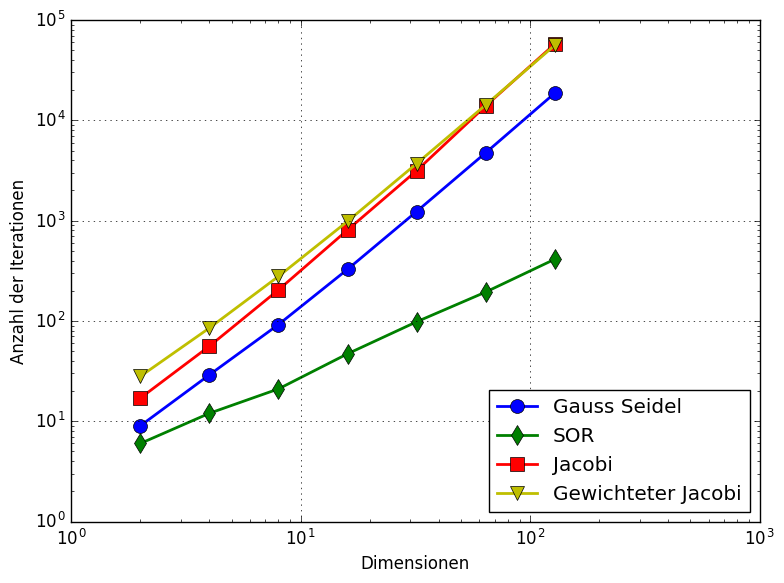
\includegraphics[width=1\textwidth]{iterationen.png}
	\caption{Vergleich der grundlegenden Verfahren}
	\label{img:Bild1}
\end{figure}
Man kann sehen das das SOR Verfahren das Verfahren ist, dass die wenigsten Iterationen braucht. Am schlechtesten schneidet das optimierte Jacobi Verfahren ab, da diese f\"ur einen speziellen Fall ist und nicht f\"ur diesen.
Es wurde best\"atigt, dass man mit mehr Informationen auch die Anzahl der Iterationen verringern kann.

\newpage

\section{Vergleich zwischen Julia und Python anhand des SOR Verfahren}
Ich habe gesehen, dass das SOR Verfahren das schnellste Verfahren ist und zudem die wenigsten Iterationen braucht. Deswegen habe ich beschlossen meinen Vergleich zwischen Julia und Python mit dem SOR Verfahren zu machen. 
Ich benutze die gleichen Vektoren wie beim Vergleich der einzelnen Verfahren.
Daf\"ur habe ich das Verfahren mit verschieden gro\ss{}en Matrizen und verschiedenen Residuen getestet. Die Gr\"o\ss{}e der Matrizen liegt zwischen 200x200 und 1600x1600. Das Residuum lasse ich von \(10^{-1}\) bis \(10^{-9}\) laufen. 
\begin{figure}[h]
	\centering
	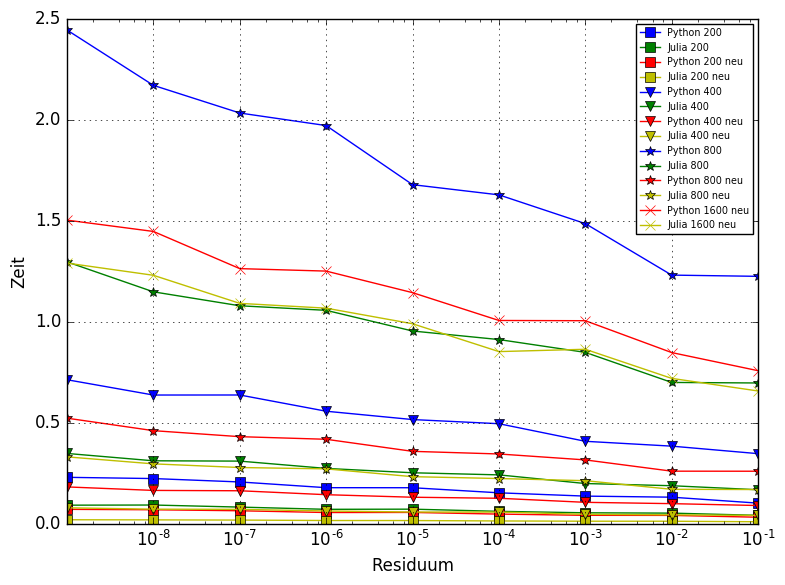
\includegraphics[width=1\textwidth]{SORneu.png}
	\caption{Vergleich SOR Verfahren aufgrund deren Matrixgroesse}
	\label{img:Bild2}
\end{figure}
Anhand dieses Diagramms, kann man sehen, dass je kleiner das Residuum ist, desto l\"anger braucht das l\"osen des LGS. Zudem kann man erkennen, dass je gr\"o\ss{}er die Matrix ist, 
desto mehr Zeit braucht der L\"oser. Hier ist auch ungef\"ahr ein quadratischer Zusammenhang zu erkennen. Es f\"allt zudem auf, dass das l\"osen ohne die LU Zerlegung bei gleicher Gr\"o\ss{}e und gleicher Iterationsanzahl 
immer langsamer ist als das l\"osen mit LU Zerlegung.Man kann au\ss{}erdem erkennen, dass das Verfahren mit LU Zerlegung in Julia am schnellsten ist. Darauf folgt das LU-Verfahren mit Python und danach das normale l\"osen in 
Julia und am langsamsten ist das l\"osen mit Python.

\newpage

\section{\"Uberpr\"ufung der Ergebnisse mithilfe des Jacobi Verfahren}
Um zu \"uberpr\"ufen, dass dieses nicht nur beim SOR Verfahren auftritt, habe ich mich entschlossen dieses mithilfe des Jacobi Verfahren zu \"uberpr\"ufen. Da aber die Test mit den gleichen Bedingungen wie beim SOR Verfahren 
sehr viel l\"anger brauchen als bei den Tests des SOR Verfahren, habe ich mich dazu entschlossen das gewichtete Jacobi Verfahren zu benutzen und den Vektor x0 als Fourier Mode zu setzen. 
Das bedeutet ich benutze eine Sinusschwingung, die durch ein Parameter k bestimmt wird, welcher abh\"angig von der Gr\"o\ss{}e n der Matrix ist. Die Sinusschwingung betrachte ich zwischen 0 und 1. 
Um verschiedene Werte f\"ur den Vektor zu bekomme, benutze ich die Werte im Abstand von 1/n+1. Hier die Formel f\"ur den i-ten Eintrag im Vektor. Ich benutze den gewichteten Jacobi, da er optimal f\"ur diese Problemstellung ist.
Je gr\"o\ss{}er man k dabei w\"ahlt, desto schneller und mit weniger Iterationen kann der iterative L\"oser das LGS l\"osen. 
\begin{figure}[h]
	\centering
	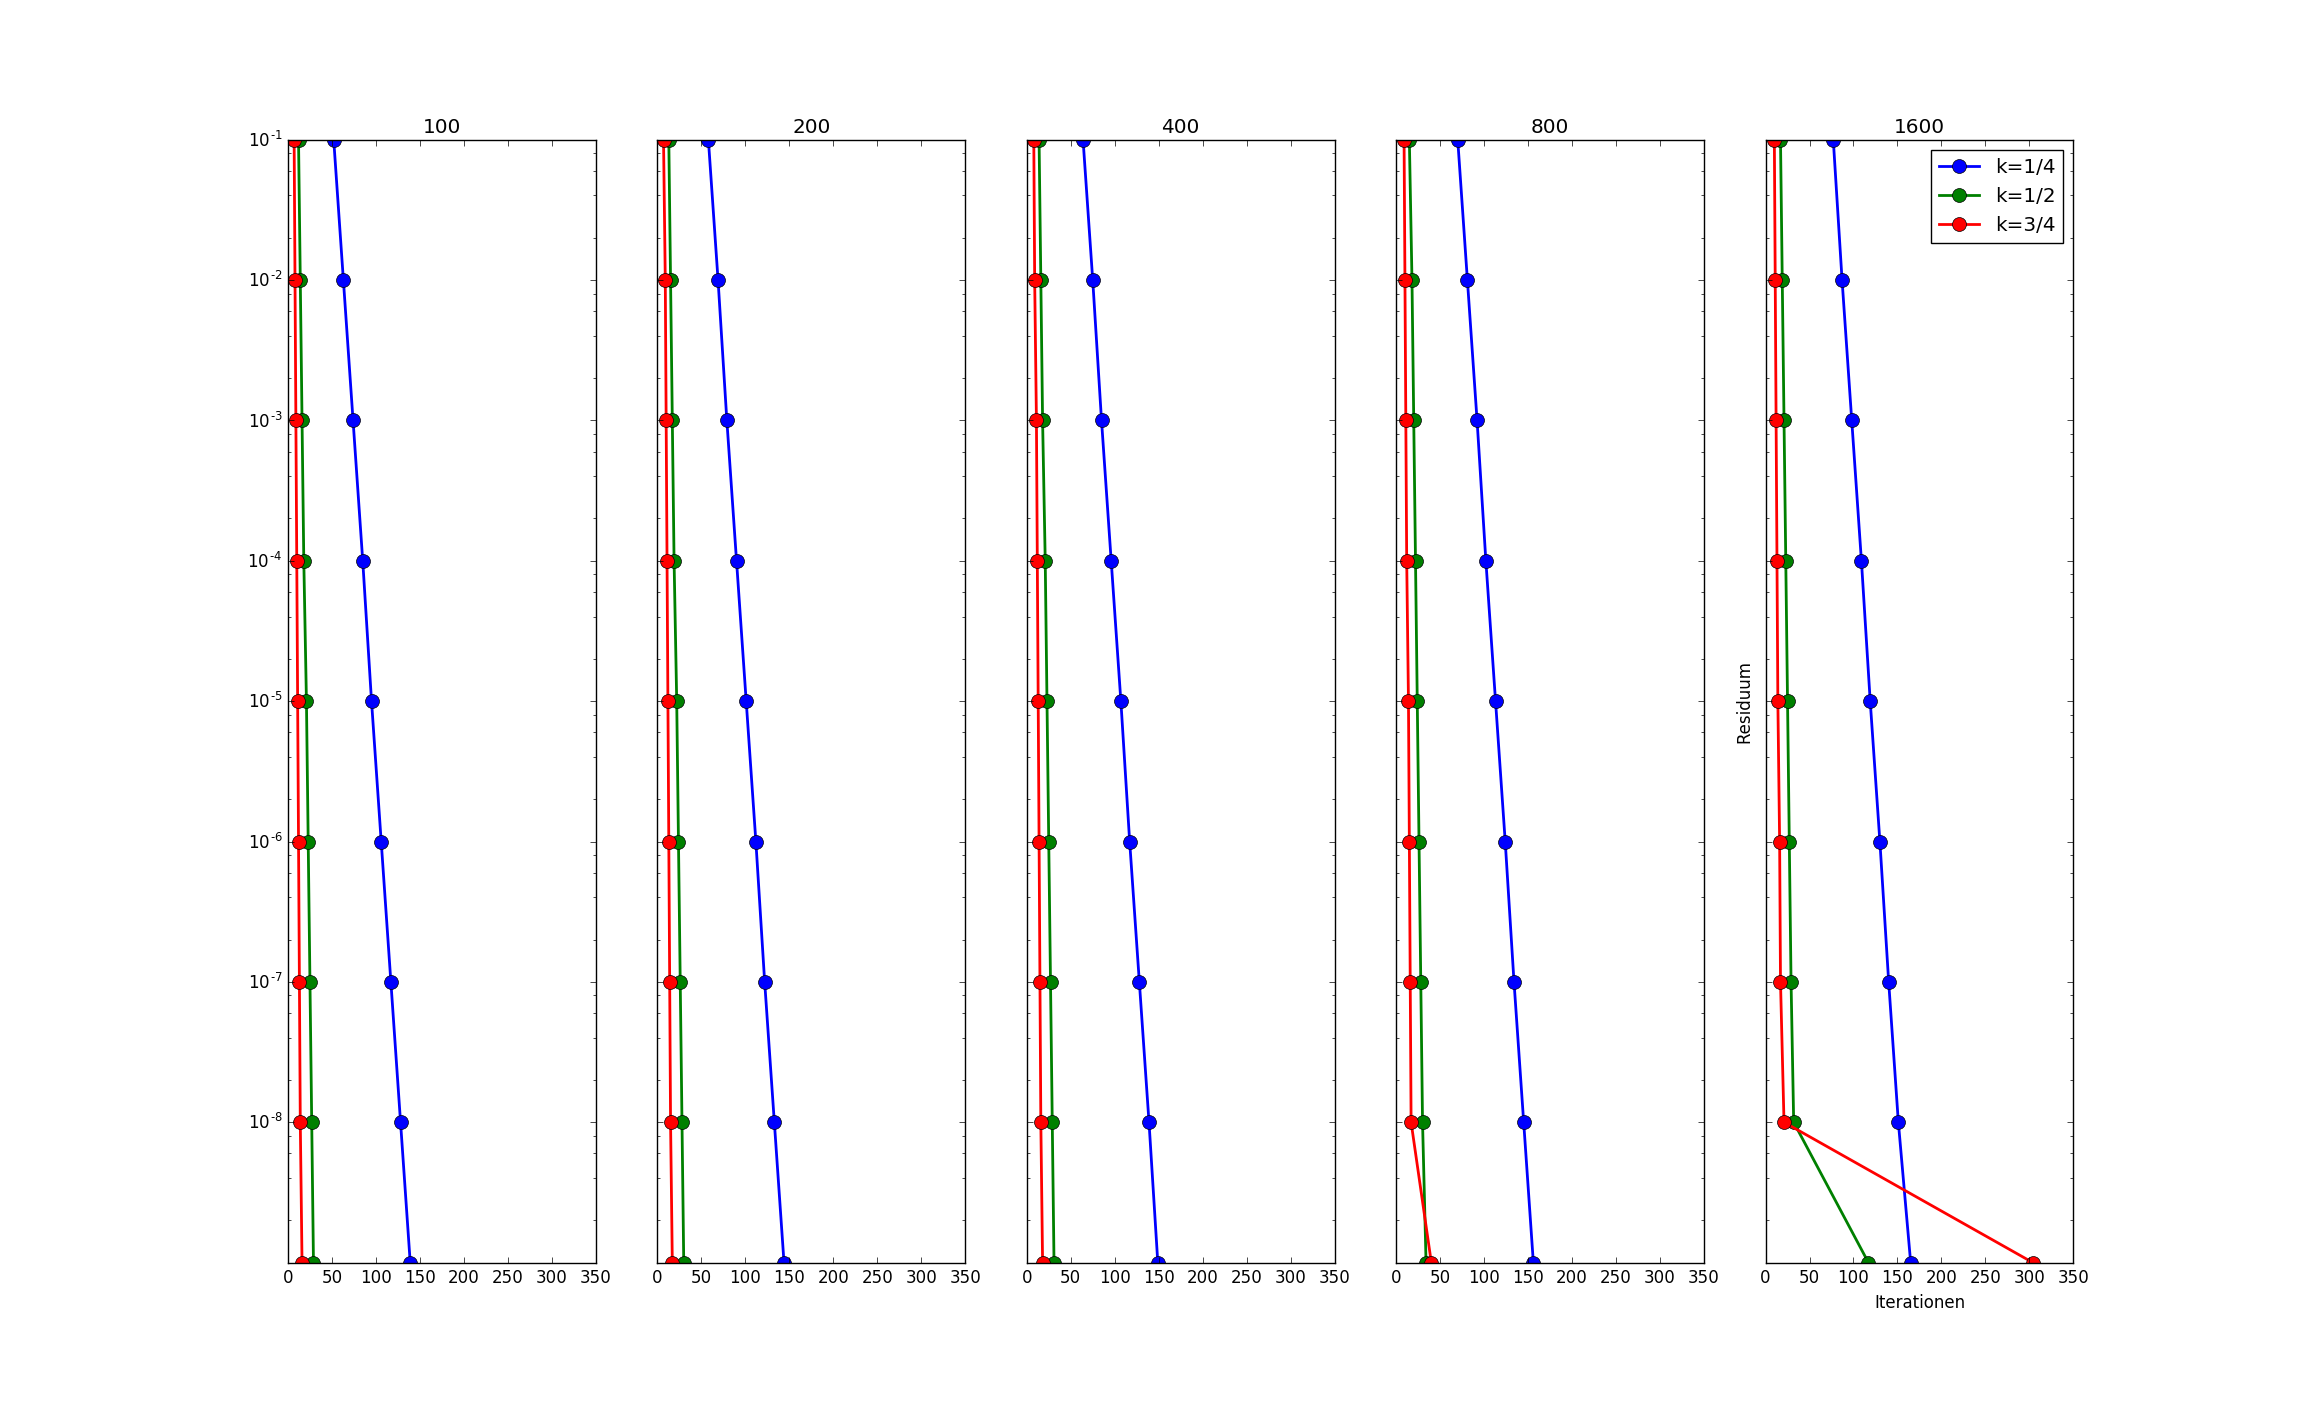
\includegraphics[width=1\textwidth]{Jacobi.png}
	\caption{Gewichteter Jacobi anhand der Matrixgroesse}
	\label{img:Bild3}
\end{figure}
Man sieht in diesem Diagramm, dass egal wie gro\ss{} man die Matrix w\"ahlt man immer die gleiche Anzahl der Iterationen, bei allen Matrixgr\"o\ss{}en f\"ur gleiches Residuum sieht. 
Wenn man allerdings die Matrizen zu gro\ss{} w\"ahlt und das Residuum zu klein, passiert etwas was ich nicht erkl\"aren kann.
Ich w\"ahle f\"ur Zeitvergleich zwischen Python und Julia k=1/10, da bei gr\"o\ss{}eren Werten der Algorithmus zu schnell wird und ich zu ungenaue Ergebnisse bekomme, da die Iterationszeit im Millisekunden Bereich liegt.
\begin{figure}[h]
	\centering
	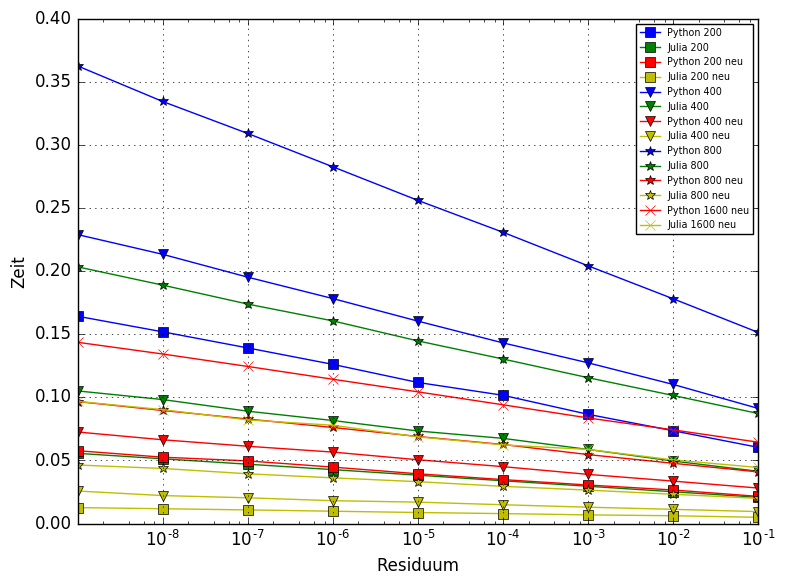
\includegraphics[width=1\textwidth]{Jacobineu.png}
	\caption{Vergleich des gewichteten Jacobi Verfahrens aufgrund der Matrixgroesse}
	\label{img:Bild4}
\end{figure}
Man kann erkennen, dass sich die Ausf\"uhrungszeiten \"ahnlich ver\"andern wie bei dem SOR Verfahren. Man kann allerdings erkennen, dass die einzelnen Graphen linearer sind als beim SOR Verfahren. Zudem f\"allt auf, dass mithilfe der 
Fourier Mode das gewichtete Jacobi Verfahren schneller ist als das SOR Verfahren.

\newpage

\section{Zwischenfazit}
Anhand der verschiedene Tests die ich durchgef\"uhrt habe, konnte ich erkennen, dass Julia eine bessere Ausf\"uhrungsgeschwindigkeit hat als Python. Die Vortest wurden somit best\"atigt. 
Zudem konnte ich erkennen, dass bei einem zuf\"alligem \(x_{0}\) das SOR Verfahren am besten geeignet ist von den hier Vorgestellten. 
Man konnte beobachten das bei kleinerem Residuum auch die Ausf\"uhrungszeit langsamer war. Zudem konnte ich best\"atigen, dass bei gr\"o\ss{}eren Matrizen der iterative L\"oser auch l\"anger braucht. 
Wenn man allerdings den \(x_{0}\) Vektor intelligent ver\"andert kann man auch andere Verfahren verschnellern. 
Bei der Implementierung von Julia ist mir aufgefallen, dass es sehr einfach ist sich in Julia einzuarbeiten. Die Dokumentation ist im Moment noch \"ubersichtlich und alle mathematischen Funktionen sind vorgegeben 
und man muss diese nicht importieren. Da Julia aber noch eine junge Sprache ist hat diese auch Nachteile. Beispielsweise musste ich oft Umwege \"uber andere Funktionen gehen.
Die Implementierung in Python dagegen war teilweise schwieriger, da die Doku sehr umfassend ist und man sich gut mit den Bibliotheken Numpy und Scipy auskennen muss, um geeignete Funktionen zu finden. 
Auf der anderen Seite hat Python eine sehr viel gr\"o\ss{}ere Community und man findet f\"ur fast jede Problemstellung schnell eine L\"osung. 
Der n\"achste Schritt wird sein diese iterativen L\"oser matrixfrei in Julia und Python zu implementieren. Zudem werde ich mich mit der Parallelisierung von Algorithmen in Julia besch\"aftigen, da dieses leichter sein soll als in Python.

\newpage

\section{Matrixfreie Implementierung }
\subsection{Warum Matrixfreie Implementierung?}
Um unser Ziel, die Parallelisierung des Jacobi Algoritmus in Julia zu erreichen, ist es notwendig das Verfahren erst in einem Vorschritt zu implementieren. Dies ist eine Matrixfreie Variante, die auf der Unabhaengigkeit 
der einzelnen Verfahrensschritte beim Jacobialgoritmus basiert. Dies ist fuer die Parralelisierung sehr wichtig. Ein weiterer Vorteil ist, das fuer diese Vorgehen weniger Speicherplatz in Anspruch genommen werden muss.

\subsection{Was bedeutet Matrixfreie Implementierung?}
Bei der Matrixfreien Implementierung geht es darum, die grossen Matritzen so darzustellen, dass diese moeglichst wenig Speicherplatz brauchen. Dies ist moeglich da wir die Gleichung \(A*x=b\) loesen wollen und \(A\) 
in unserem Fall die Matrix ist, die bei der Diskretisierung des Laplace-Operators mit Finiten Differenzen zweiter Ordnung mit Dirichlet-Randbedingungen in einer Dimension ensteht. Wichtig an dieser Matrix ist aber, 
dass diese nur Eintraege auf der Diagonalen und den beiden Nebendiagonalen hat und dass alle Eintraege auf einer Diagonalen gleich sind.
Dies macht es mir moeglich die Matrix als Stencil abzuspeichern. Das bedeutet in diesem Fall das die Matrix folgendermassen abgespeichert wird:

\zitat{matrix = [-((n+1)*(n+1)), 2*((n+1)*(n+1)), -((n+1)*(n+1))]}

Diese Matrix bezeichne ich im weiteren mit \(a\).
Das bedeutet auch das ich den Algorithmus dem hingehend veraendern muss, sodass dieser nicht mehr auf die einzelnen Elemente der Matrix \(A\) zugreifen kann, sondern immer nur auf diese drei Elemente.
Alle anderen Vektoren sollen sich aber nicht veraendern. Das Ergebnis soll auch das gleiche sein.

\newpage

\subsection{Jacobi matrixfrei}
Um zur Matrixfreien Methode zu kommen muss man betrachten, was in jeder Zeile einer Iteration bei der Matrixmultiplikation vor sich geht. Bei der Multiplikation von Matrix mit einem Vektor wird fuer jeden Wert \(b_{n}\) 
im Ergebnisvektor die entsprechende Zeile in der Matrix mit dem Vektor verrechnet. Da in diesem Fall die Matrix sehr speziell ist und nur Nulleintr?ge hat au?er auf der Hauptdiagonalen und den beiden Nebendiagonalen. 
Um den Wert $b_{n}$ im Ergebnisvektor zuberechnen sind also nur die drei Eintaege \(x_{n-1}, x_{n}\) und \(x_{n+1}\)wichtig. Diese werden mit dem entsprechenden Wert multipliziert.

Die Formel fuer den Jacobi Algorithmus ist folgende: 
\begin{equation}
  x_{k+1}=w(I-D^{-1}A)x_{k}+D^{-1}b
\end{equation}

Diese kann man umstellen damit erleichter fuer das matrixfreie Rechnen wird: 
\begin{equation}
x_{k+1}=(1-w)x_{k}+-wD^{-1}*(Ax_{k}-b)
\end{equation}
\begin{equation}
\Rightarrow x_{k+1}=(1-w)x_{k}+\frac{w}{a_{ii}}(b-\sum_{j \neq i}a_{ij}x_{k,j})
\end{equation}

Wenn man jetzt daran denkt, was Matrixfreies implementieren bedeutet sieht man, das man die die Gleichung fuer jedes \(x_{k+1,i}\) umstellen kann. Man muss jedoch implementionsseitig bedenken, dass es eine Kopie
des \(x_{k}\) geben muss, weil wir auch die alten Eintraege des \(x_{k}\).

Die Implementierung sieht also folgendermassen aus:
\zitat{x[i]= (1-w)*xalt[i]+((w/matrix[1])*(b[i]-(matrix[0]*xalt[i-1]+matrix[2]*xalt[i+1])))}

Ich teste die matrixfreie Variante mit der Fouriermode fuer k=40\% bei einem Residuum=0.1. Ich waehle den Parameter w=2/3, da so ein optimales Ergebnis herauskommt. Ich teste dieses in Julia und Python und vergleiche dieses mit 
der Matriximplementierung und Der Matriximplementierung die mit dem LU Verfahren arbeitet. Ich betrachte dabei die Zeit die eine Iteration braucht im Verhaeltnis zur Matrixgroesse, welches bedeutet, wie lange der Computer braucht 
um ein besseres \(x_{k}\) zu berechnen. Die Betrachtung der Zeit pro Iteration ist notwendig, um das Verfahren mit dem SOR Verfahren zu vergleichen und um die Veraenderungen in der Matrixgroesse besser nachvollziehen zu koennen. 
Man koennte beim Jacobi Verfahren auch die absolute Zeit betrachten, da die Anzahl der Iterationen bei konstantem k konstant bleibt. Ich ueberpruefe das Verfahren anhand ihrer Iterationszahlen.

\begin{figure}[h]
	\centering
	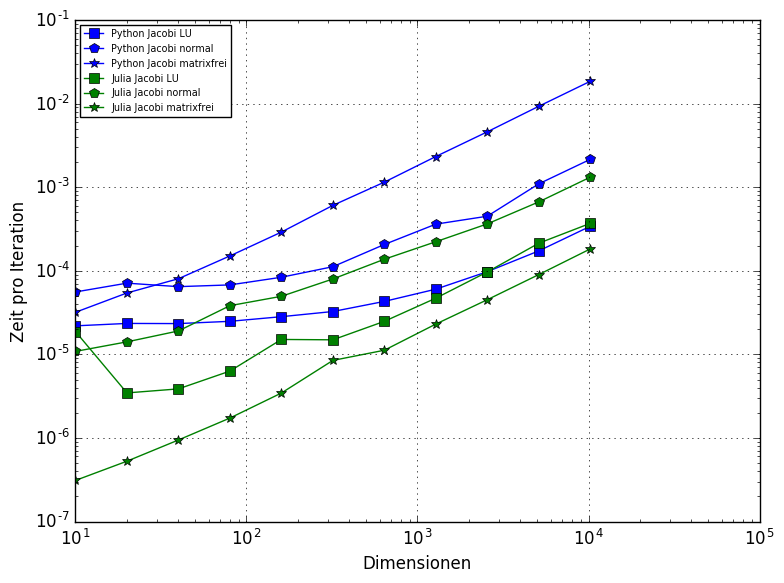
\includegraphics[width=1\textwidth]{jacobimatrixfrei.png}
	\caption{Vergleich Jacobi matrixfrei}
	\label{img:Bild5}
\end{figure}

Man kann erkennen, dass das schnellste Verfahren die matrixfreie Implementierung in Julia ist und das langsamste Verfahren die Matrixfreie Implementierung in Python. Die Matrixbasierten Implementierungen liegen zwischen beiden matrixfreien Varianten. 
Es ist erstaunlich das bei grossen MAtritzen die LU Variante in Python die zweitschnellste wird, dies hatten wir in den vorherigen Tests nicht gesehen.

\newpage

\subsection{SOR matrixfrei}}
Die Allgemeine Formel fuer das SOR Verfahren ist: 
\begin{equation}
x_{k+1}=(1-w)x_{k}+\frac{w}{a_{ii}}(b-\sum_{j<i}a_{ij}x_{k+1 j}-\sum_{j>i}a_{ij}x_{k+1 j})
\end{equation}
Aufgrund der Struktur des SOR Verfahren:

\zitat{x[i]= (1-w)*x[i]+((w/matrix[1])*(b[i]-(matrix[0]*x[i-1]+matrix[2]*x[i+1])))}

\par Ich teste das SOR Verfahren mithilfe der Fouriermode mit k=40\% bei einem Residuum=0.01, damit ich dieses mit dem Jacobi Verfahren vergleichen kann. Auch hier teste ich in Julia und Python und benutze zum vergleichen die 
matrixbasierten Varianten. Ich muss hier den Parameter w=1 waehlen, da ich sonst keinen Trend in den Iterationszahlen feststellen kann. Damit ist das SOR Verfahren hier im Grunde das Gauss Seidel Verfahren ist. 
Trotzdem sind die Iterationszahlen hier nicht konstant deswegen ist hier vor allem die Zeit pro Iteration wichtig.

\begin{figure}[h]
	\centering
	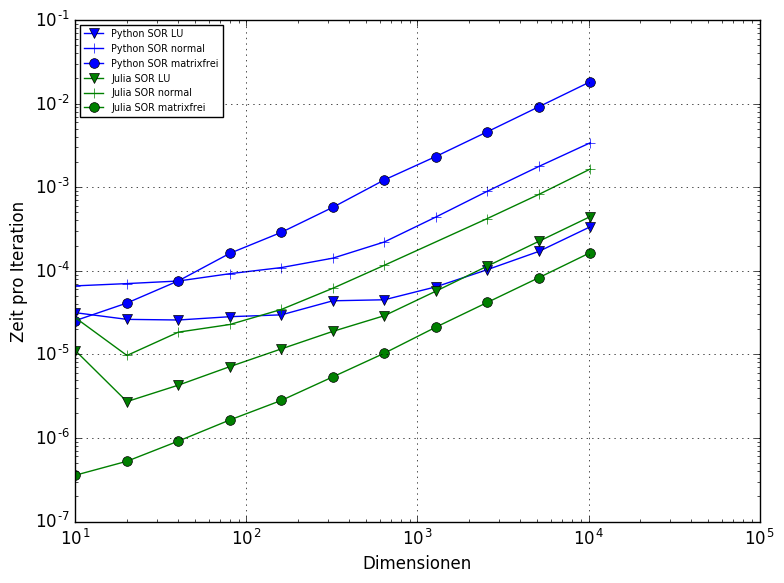
\includegraphics[width=1\textwidth]{SORmatrixfrei.png}
	\caption{Vergleich SOR matrixfrei}
	\label{img:Bild6}
\end{figure}

Man kann erkennen, dass das schnellste Verfahren die matrixfreie Implementierung in Julia ist und das langsamste Verfahren die Matrixfreie Implementierung in Python. Die Matrixbasierten Implementierungen liegen zwischen beiden matrixfreien Varianten. 

\subsection{Vergleich der Matrixfreien Varianten}
Man kann erkennen, dass die Verfahren vor allem die Matrixbasierten Varianten in etwa gleich viel Zeit brauchen, was erstaunlich ist, da im Jacobi Verfahren ein Schritt mehr gemacht werden muss und ein Vektor kopiert werden muss. 
Dies kann aber nicht vermieden werden. Wenn mann die Gesamtzeiten betrachtet, kann man erkennen, das das Jacobi Verfahren an sich schneller ist, da dieses weniger Iterationen benoetigt.

\newpage

\section{Fazit}
Schlussendlich kann ich sagen, dass die Matrixfreien Varianten von der Laufzeit her in Julia und in Python sehr unterschiedlich sind. In Julia ist diese Variante sehr schnell, wohingegen in Python diese Variante sehr langsam ist.

% das ist wohl jetzt das Ende des Dokumentes
\end{document}
